\documentclass[]{article}
%%% Document layout & text formatting
\usepackage[margin=0.75in]{geometry}
\usepackage[english]{babel}
\usepackage[utf8]{inputenc}

%%% Figures, tables, plots support
\usepackage{graphicx}
\usepackage{caption}
\captionsetup{justification=centering,font={small,sf}}
\usepackage{subcaption}
\usepackage[dvipsnames]{xcolor}
%\usepackage{listings}
\usepackage{color}

\definecolor{mygreen}{rgb}{0,0.6,0}
\definecolor{mygray}{rgb}{0.5,0.5,0.5}
\definecolor{mymauve}{rgb}{0.58,0,0.82}

\lstset{
  backgroundcolor=\color{white},   % choose the background color; you must add \usepackage{color} or \usepackage{xcolor}; should come as last argument
  basicstyle=\footnotesize,        % the size of the fonts that are used for the code
  breakatwhitespace=false,         % sets if automatic breaks should only happen at whitespace
  breaklines=true,                 % sets automatic line breaking
  captionpos=b,                    % sets the caption-position to bottom
  commentstyle=\color{mygreen},    % comment style
  deletekeywords={...},            % if you want to delete keywords from the given language
  escapeinside={\%*}{*)},          % if you want to add LaTeX within your code
  extendedchars=true,              % lets you use non-ASCII characters; for 8-bits encodings only, does not work with UTF-8
  firstnumber=1,                   % start line enumeration with line 1000
  frame=single,	                   % adds a frame around the code
  keepspaces=true,                 % keeps spaces in text, useful for keeping indentation of code (possibly needs columns=flexible)
  keywordstyle=\color{blue},       % keyword style
  language=Python,                 % the language of the code
  morekeywords={*,...},            % if you want to add more keywords to the set
  numbers=left,                    % where to put the line-numbers; possible values are (none, left, right)
  numbersep=5pt,                   % how far the line-numbers are from the code
  numberstyle=\tiny\color{mygray}, % the style that is used for the line-numbers
  rulecolor=\color{black},         % if not set, the frame-color may be changed on line-breaks within not-black text (e.g. comments (green here))
  showspaces=false,                % show spaces everywhere adding particular underscores; it overrides 'showstringspaces'
  showstringspaces=false,          % underline spaces within strings only
  showtabs=false,                  % show tabs within strings adding particular underscores
  stepnumber=1,                    % the step between two line-numbers. If it's 1, each line will be numbered
  stringstyle=\color{mymauve},     % string literal style
  tabsize=4,	                   % sets default tabsize to 2 spaces
  title=\lstname                   % show the filename of files included with \lstinputlisting; also try caption instead of title
}
\usepackage[cache=false]{minted}
\usemintedstyle{vs}

%%% Maths
\usepackage{amsmath}
\usepackage{amssymb}
\usepackage{wasysym}
\usepackage{siunitx}
\sisetup{separate-uncertainty = true, multi-part-units = brackets}
% fractions as powers
\usepackage{xfrac}

% differential (needs upright, not slanted d)
\newcommand{\dd}{\mathop{}\!\mathrm{d}}
% boldface vectors
\let\OLDvec\vec
\renewcommand{\vec}[1]{\boldsymbol{#1}}
% some constants
\newcommand{\rhoCentre}{\rho_\mathrm{c}}
\newcommand{\fermiMtm}{p_\mathrm{F}}
\newcommand{\massElectron}{m_\mathrm{e}}
\newcommand{\massProton}{m_\mathrm{p}}
\newcommand{\gravconst}{\mathrm{G}}


%%% References
% bibliography
%\usepackage{bibtex}
\usepackage[square,sort,comma,numbers]{natbib}
\setcitestyle{authoryear,open={(},close={)}}
\let\OLDthebibliography\thebibliography
\renewcommand\thebibliography[1]{
  \OLDthebibliography{#1}
  \setlength{\parskip}{3pt}
  \setlength{\itemsep}{0pt plus 0.3ex}
}

% hyperlinks
\usepackage{hyperref}
\hypersetup{
	colorlinks=true,
	linkcolor=RoyalBlue,
	filecolor=magenta,
	urlcolor=Salmon,
	citecolor=RoyalBlue,
}
% more options on https://www.overleaf.com/learn/latex/hyperlinks

%%% Other new commands
% names of runs
\newcommand{\eulerOne}{\textsc{Euler1}}
\newcommand{\eulerTwo}{\textsc{Euler2}}
\newcommand{\heun}{\textsc{Heun}}
\newcommand{\rkFour}{\textsc{RK4}}

%\usepackage{showframe}

\begin{document}

% \title{This is a title}
% \author{Lyubomir Shoylev, \texttt{shil5377}}

% \maketitle

\begin{center}
	\Large{\textbf{CO31: Structure of white dwarf stars}\\
	\vspace{1em}
	\large{Lyubomir Shoylev, \texttt{shil5377}}\\ \href{mailto:me@example.com}{\texttt{lyubomir.shoylev@st-hildas.ox.ac.uk}}}\\
	\large{St Hilda's College}\\
	\today
\end{center}

\begin{abstract}
	In an experiment, we attempt to study the structure of white dwarf stars. We give a short derivation of the differential equations describing a white dwarf in equilibrium under some assumptions about the matter. Then we introduce the computational approach of our solution and decide on parameters for the calculation. We present the dependence of radius and mass of white dwarfs on central density, as well as the relationship between them, which gives rise to the \emph{Chandrasekhar mass limit}. We discuss some of its implications, after which we present a summary of the experiment and comment on further improvements.
\end{abstract}

\section{Introduction}
	The goal of this experiment is to study the internal structure of white dwarf stars. They are one possible end state in the life cycle of stars. What is particular about white dwarf stars is that the matter they are composed of is different from the matter in a usual star similar to the Sun. While in a usual stable star the equilibrium is largely supported by fusion energy and the pressure of the plasma, a white dwarf star has reached the end of the fusion processes, and the equilibrium is supported by electron degeneracy pressure, making the star extremely dense; for example, a white dwarf of one solar mass is about the size of Earth. In this report, we will first derive the coupled differential equations for mass and density in a spirit similar to \cite{OxfPhys2020} and \cite{Chandrasekhar1984} in Section \ref{sec:theroy-white-dwarfs}. Then, in Section \ref{sec:numerical-approach}, we develop the numerical method used to solve the coupled equations. Results and discussion take place in Section \ref{sec:results-and-discussion}. Finally, we give a summary of the experiment and possible improvements in Section \ref{sec:summary}.
	%======================= decide if the last sentence is ok

\section{Theory of white dwarf stars}\label{sec:theroy-white-dwarfs}
	Stars are astronomical objects with ellipsoid shape made up of heated plasma. The force of gravity tries to compress the ball, holding the matter together, while the gaseous plasma opposes gravity with the pressure it exerts. When the two forces balance each other out, the star is in hydrostatic equilibrium. In usual stars, pressure is due to the gas and the radiation. In white dwarf stars, however, the densities are far greater than the ones found in usual stars, and matter behaves differently. All electrons are no longer bound to atoms and are free to roam. The behaviour can approximately be modelled by a Fermi gas of electrons at zero Kelvin (i.e. fully degenerate state). Hence, the pressure ensuring the equilibrium is the degeneracy pressure of the electrons.
	% TODO more context about white dwarfs as evolutionary states of massive stars.

\subsection{Equation of equilibrium}\label{subsec:test}
	%		- Equation of equilibrium
	Assume the star is spherically symmetric, in equilibrium, non-rotating, and the effect of magnetic fields is negligible. Therefore, all properties depend only on the distance to the centre of the star, $r$. The gravitational force on a small volume of matter with area $\dd A$ and radial height $\dd r$ is:
	\begin{equation}
		F_\mathrm{G} = - \frac{G m\left(r\right) \dd m}{r^2},
	\end{equation}
	where $m\left(r\right)$ is the mass of the star contained up to $r$, $\dd m = \dd A \dd r \rho \left(r\right)$ is the mass of the small volume, and the density $\rho \left(r\right)$ was assumed constant (negative sign because it pulls towards the centre). The force due to the pressure is the difference of the forces at $r$ and $r + \dd r$:
	\begin{equation}
	F_\mathrm{P} = \left( P\left(r\right) - P\left(r + \dd r\right)\right) \dd A.
	\end{equation}
	For a star in equilibrium, the two forces balance each other out, i.e. $F_\mathrm{G} + F_\mathrm{P} = 0$. After rearranging, we get:
	\begin{equation} \label{eqn:hydrostat-equil}
		\frac{\dd P(r)}{\dd r} = \frac{P\left(r + \dd r\right) - P\left(r\right)}{\dd r} = - \frac{G \rho(r) m(r)}{r^2}.
	\end{equation}
	We can rewrite the hydrostatic equilibrium by using the chain rule:
	\begin{equation}
		\frac{\dd P(r)}{\dd r} = \frac{\dd P}{\dd \rho} \frac{\dd \rho}{\dd r},
	\end{equation}
	so equation \eqref{eqn:hydrostat-equil} becomes:
	\begin{equation}\label{eqn:hydrostat-equil-rhor}
		\frac{\dd \rho}{\dd r} = - \frac{\dd \rho}{\dd P} \frac{G \rho(r) m(r)}{r^2}.
	\end{equation}

	On the other hand, the equation for the inscribed mass is:
	\begin{equation}\label{eqn:mass-dEq}
		m(r) = \int_0^r \dd r' 4 \pi^2 r' \rho\left(r'\right) \quad \Rightarrow \quad \frac{\dd m}{\dd r} = 4 \pi r^2 \rho(r)
	\end{equation}
	We are now left with two coupled differential equations, \eqref{eqn:hydrostat-equil-rhor} and \eqref{eqn:mass-dEq}. The last task before obtaining the full equation is to determine $\frac{\dd P}{\dd \rho}$ which depends on the equation of state.

\subsection{Equation of state}
	%		- Equation of state - non-relativistic and relativistic (derive to common form)
	We assume the star is made up primarily of heavy $^{56}$Fe nuclei and their electrons. The nuclei carry most of the mass and little of the pressure, while the opposite is true for the electrons. Since \emph{very~high} densities are considered, we can approximate that the nuclei are stationary while the electrons move freely, not bound to any nuclei. A good model for the freely moving electron gas is the free Fermi gas at $T = \SI{0}{K}$. This is the fully degenerate state, in which electrons fill all energy (momentum) levels up to the Fermi energy (momentum).

	Fermions obey the Pauli exclusion principle, therefore each energy level is $2S + 1$ degenerate, where $S = \frac{1}{2}$ in the case of electrons. This degeneracy factor multiplies gives the density function:
	\begin{equation}
		g(k) = \frac{2S + 1}{2 \pi^2} V k^2,
	\end{equation}
	where $k$ is the wave vector of particles and $V$ is the volume of the system. The number density of particles can therefore be written as:
	\begin{equation}
		n = \frac{N}{V} = \frac{1}{V} \int_0^{k_\mathrm{F}} \dd k \, g(k) = \int_0^{k_\mathrm{F}} \dd k \frac{2S + 1}{2 \pi^2} k^2.
	\end{equation}
	Here we integrate up to $k_\mathrm{F}$ where this is given by $\fermiMtm = \hbar k_\mathrm{F}$ and $\fermiMtm$ is the Fermi momentum. Rewrite the above equation in terms of $p$:
	\begin{equation}\label{eqn:number-density}
		n = \int_0^{\fermiMtm} \dd p \frac{2S + 1}{2 \pi^2 \hbar^3} p^2 = \int_0^{\fermiMtm} \dd p \frac{8 \pi}{h^3} p^2 = \int_0^{\fermiMtm} \dd p \, n(p) = \frac{\massElectron8 \pi}{h^3} \fermiMtm^3
	\end{equation}
	where we define $n(p) \dd p$ as the number of electrons per unit volume with momentum between $p$ and $p + \dd p$.

	Pressure, on the other hand, is given by the kinetic expression:
	\begin{equation}\label{eqn:pressure-int}
		P = \frac{1}{3} \int_0^{\fermiMtm} p v_p n(p) \dd p.
	\end{equation}
	At this point we need to differentiate between non-relativistic and relativistic cases - $v_p$ has a different value in the two cases:
	\begin{equation}
		v_p = \begin{cases}
			\frac{p}{\massElectron} & \text{ in the non-relativistic case} \\
			\frac{pc^2}{\sqrt{p^2c^2 + \massElectron^2 c^4}} & \text{ in the relativistic case}
		\end{cases}.
	\end{equation}

	Let us first work out the answer in the non-relativistic case. The integral becomes $\text{const} \times \int p^4 \dd p$, so the pressure becomes:
	\begin{equation}\label{eqn:pressure-non-rel}
		P_\mathrm{non} = \frac{8 \pi}{15 h^3 \massElectron} \fermiMtm^5.
	\end{equation}
	For the relativistic case, rather than do the integral for P involving hyperbolic functions, differentiate \eqref{eqn:pressure-int} by parts:
	\begin{equation}\label{eqn:pressure-rel}
		\frac{\dd P_\mathrm{rel}}{\dd \rho} = \frac{\dd P_\mathrm{rel}}{\dd \fermiMtm} \frac{\dd \fermiMtm}{\dd \rho}, \quad \frac{\dd P_\mathrm{rel}}{\dd \fermiMtm} = \frac{8\pi}{3h^3}\frac{\dd}{\dd \fermiMtm}\int_0^{\fermiMtm} \frac{p^4 c^2}{\sqrt{p^2c^2 + \massElectron^2 c^4}} \dd p = \frac{8\pi}{3h^3} \frac{\fermiMtm^4 c}{\sqrt{\fermiMtm^2c^2 + \massElectron^2 c^4}}.
	\end{equation}
	We can collect the derivative of \eqref{eqn:pressure-non-rel} and the result of \eqref{eqn:pressure-rel}:
	\begin{equation}\label{eqn:pressure-both}
		\frac{\dd P}{\dd \rho} = \frac{\dd \fermiMtm}{\dd \rho}\frac{8 \pi}{3 h^3 \massElectron} \fermiMtm^4 \times \begin{cases}
			1 & \text{ in the non-relativistic case} \\
			\left(1 + \frac{\fermiMtm^2}{\massElectron^2 c^2}\right)^{-\sfrac{1}{2}} & \text{ in the relativistic case}
		\end{cases}.
 	\end{equation}

	What is left is expressing $\fermiMtm (\rho)$ to complete the equation of state in the form needed by \eqref{eqn:hydrostat-equil-rhor}. The relation between density and number density can be stated as $\rho = \mu_\mathrm{e} \massProton n$, where $\mu_\mathrm{e}$ is the mean molecular weight per electron and $\massProton$ is the mass of 1 proton. In our case, we can approximate $\mu_\mathrm{e} \approx 2$. Using this relation and \eqref{eqn:number-density}, we arrive at:
	\begin{equation}\label{eqn:fermi-mtm}
		\fermiMtm = \left( \frac{h^3}{8 \pi} n \right)^{\sfrac{1}{3}} = \left( \frac{h^3}{16 \pi \massProton} \rho\right)^{\sfrac{1}{3}} \quad \Rightarrow \quad \frac{\dd \fermiMtm}{\dd \rho} = \frac{1}{3} \left( \frac{h^3}{16 \pi \massProton}\right)^{\sfrac{1}{3}} \rho^{-\sfrac{2}{3}}
	\end{equation}

\subsection{The limiting mass}
	The limiting case of ultra-relativistic electrons can be obtained by setting $v_p = c$ (i.e. taking the limit $pc \gg \massElectron c^2$) in \eqref{eqn:pressure-int} to arrive at the equation of state:
	\begin{equation}
		P_\mathrm{ultra} = \frac{p \pi}{3 h^3} \int_0^{\fermiMtm} p^3 c \dd p = \frac{2 \pi c}{3 h^3} \fermiMtm^4.
	\end{equation}
	As noted in \cite{Chandrasekhar1984}, this leads to a specific equation for the mass with a well-specified value $M_\mathrm{lim} = 5.76 \mu_{\mathrm{e}}^{-2} M_{\astrosun}$, where $M_{\astrosun}$ is one solar mass; this limit is equivalent to infinite mean density and zero radius of the star. In the approximation made above the limiting mass is $M_\mathrm{lim} \approx 1.435 M_{\astrosun}$. This will be ``experimentally'' verified by the computations presented in Section \ref{sec:results-and-discussion}. We can draw two important conclusions from this fact: first, there is an upper limit to masses of degenerate stars in the later stages of evolution; and second, we cannot predict the end evolutionary state of stars with mass $ M > M_\mathrm{lim}$ in this physical framework (we expand more on this in Section \ref{sec:results-and-discussion}).

\section{Numerical approach}\label{sec:numerical-approach}
	%Section 3 - Numerical approach
	To find the radius and mass of the star as a function of its central density, we will numerically integrate the coupled system. The distance $r$ at which $\rho (r=R) \approx 0$ is where the star ends; the mass is, therefore, $m(R)$ where $m(r)$ is the inscribed mass, as defined in \eqref{eqn:mass-dEq}. Physically, we can consider solving the equation as an initial value problem. First, write the coupled system in vector form:
	\begin{equation}
		\vec{y} = \begin{pmatrix}
			\rho \\
			m
		\end{pmatrix},
	\end{equation}
	and the derivatives of its members with respect o $r$ given by \eqref{eqn:hydrostat-equil-rhor} and \eqref{eqn:mass-dEq}. Then, for a given central density $\rhoCentre$ the initial condition for the mass is specified by $m(\delta r) = \frac{4}{3} \pi (\delta r)^3 \rhoCentre$ for some small distance from the centre $\delta r$: this is done so we can start the calculations ($r=0$ would give initial zero mass and the derivative is therefore zero). We will set up the equation solver so that this $\delta r$ is the step size in radial distance. The source code can be found in Appendix \ref{app:source-code}.

\subsection{Why integration?}\label{subsec:why-integ}
	%		- Why integration
	Since we have an initial value problem, the underlying idea is the following: rewrite the derivatives as fractions of finite differences, and get $\Delta \vec{y} = \frac{\dd \vec{y}(x)}{\dd x} \Delta x$. This is the change in $\vec{y}$ when we step through by $\Delta x$. When the step is very small, the approximation is very good, i.e. $\lim_{\Delta x \rightarrow \dd x} \Delta \vec{y} = \dd \vec{y}$.

	The basic idea boils down to the most elementary such method, the explicit Euler's method:
	\begin{align}
		\vec{y}_\mathrm{n+1} &= \vec{y}_\mathrm{n} + h \vec{f}(x_\mathrm{n}, \vec{y}_\mathrm{n})\\
		x_\mathrm{n+1} &= x_\mathrm{n} + h, \nonumber
	\end{align}
	where the vector function is just $\vec{f} = \frac{\dd \vec{y}(x)}{\dd x}$ i.e. the slope at $x_\mathrm{n}$ and $h = \Delta x$. This is a first order method: the local error is $\sim h^2$ and the global error, therefore, is $\sim h$. This method has only one computation of the derivative and is therefore very fast, but also very inaccurate.

	A similar explicit second order method is Heun's method (trapezoid rule):
	\begin{align}
		\vec{y}_\mathrm{n+1} &= \vec{y}_\mathrm{n} + \frac{1}{2} h \Big(\vec{f}(x_\mathrm{n}, \vec{y}_\mathrm{n}) + \vec{f}\big(x_\mathrm{n} + h, \vec{y}_\mathrm{n} + \vec{f}(x_\mathrm{n}, \vec{y}_\mathrm{n})\big)\Big)\\
		x_\mathrm{n+1} &= x_\mathrm{n} + h, \nonumber
	\end{align}
	Here the local error is $\sim h^3$ and the global error therefore is $\sim h^2$.

	The method we will later use to compute properties of white dwarf stars is the 4th order Runge-Kutta (RK4) method. It features four evaluations of the derivative and a global error $\sim h^4$, offering a balance between computational time and accuracy. This method takes values for the slope at four different positions and estimates the step size by a weighted average of these four steps. In equations:
	\begin{align*}
		\vec{k_1} &= h \vec{f}(x_\mathrm{n}, \vec{y}_\mathrm{n})\\
		\vec{k_2} &= h \vec{f}\left(x_\mathrm{n} + \frac{1}{2} h, \vec{y}_\mathrm{n} + \frac{1}{2}\vec{k_1}\right)\\
		\vec{k_3} &= h \vec{f}\left(x_\mathrm{n} + \frac{1}{2} h, \vec{y}_\mathrm{n} + \frac{1}{2}\vec{k_2}\right)\\
		\vec{k_4} &= h \vec{f}(x_\mathrm{n} + h, \vec{y}_\mathrm{n} + \vec{k_3}).
	\end{align*}
	Finally, the new position is calculated as:
	\begin{equation}
		\vec{y}_\mathrm{n+1} = \vec{y}_\mathrm{n} + \frac{1}{6} \vec{k_1} + \frac{1}{3} \vec{k_2} + \frac{1}{3} \vec{k_3} + \frac{1}{6} \vec{k_4}.
	\end{equation}
	The RK methods family gives approximate solutions to $N$th order by varying the weights in the $\vec{k}$ expressions and the final expression to match coefficients in the Taylor expansion.

	We should note that the equation to be solved might prove difficult to solve, even using RK4. These equations are often called \emph{stiff} and in constructing their solutions more precaution needs to be taken, for example by using implicit or semi-implicit methods.

\subsection{Comparison of methods}
	In this section, we compare the stability/accuracy of the three methods presented in Section \ref{subsec:why-integ}. For the task, we will try to integrate a solution of the simple harmonic oscillator (SHO), namely:
	\begin{equation}
		\ddot{x} + \omega^2 x = 0, \quad \text{ with solution } \quad x = x_0 \cos(\omega t)
	\end{equation}
	where we choose $x_0 = 1$ and $\omega = 2 \pi$ so the period of oscillations is \SI{1}{s}. From some initial runs integrating the white dwarf equation, we are aware that the number of intervals relevant to us is on the order of $10^{6}$, so we choose to compare the two methods on this scale (more discussion on the topic in Section \ref{subsec:convergence}).

	The runs are split into two groups. The first group is with $10^6$ time intervals of length \SI{1}{ms} for the three methods; denote the results from these runs by \eulerOne{}, \heun{}, and \rkFour{}, respectively. The second group is $10^7$ time intervals of length \SI{0.1}{ms} for the Euler method to cover the same total time interval; denote results by \eulerTwo{}. Additionally, we will consider the energy in the system:
	\begin{equation}
		E = \frac{\dot{x}^2}{2} + \frac{\omega^2 x^2}{2}.
	\end{equation}
	When the method over/underestimates the correction, the effect will build up and change the total energy, which is equivalent to the change in amplitude.

	\begin{figure}[!htb]
		\hfill
		\begin{subfigure}[t]{0.48\textwidth}
			\centering
			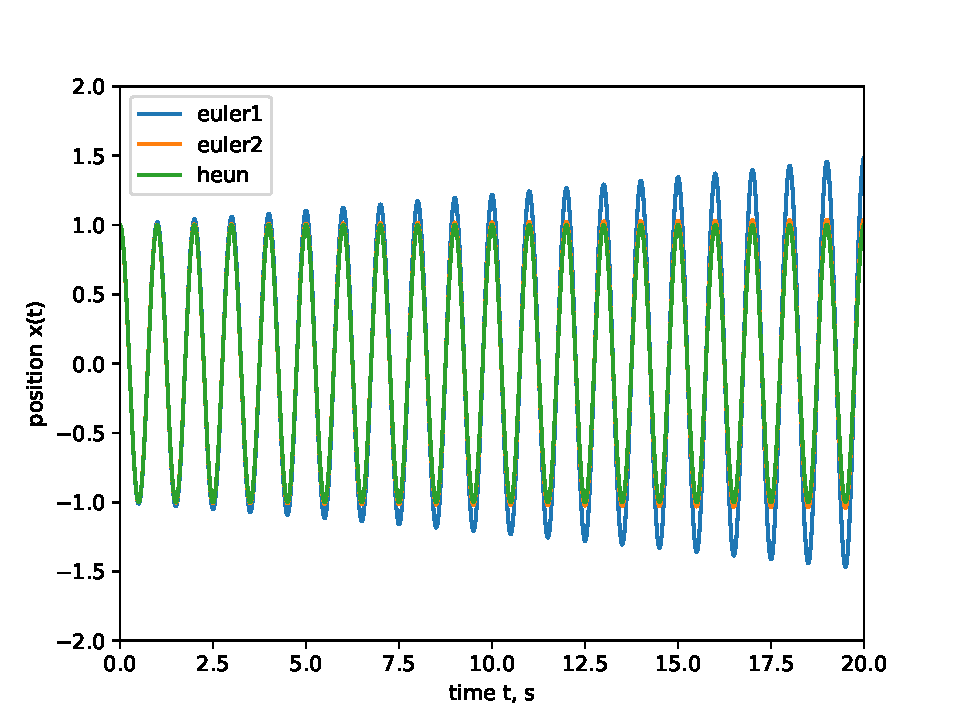
\includegraphics[width=\textwidth]{figures/eul12+heun.pdf}
			\caption{Position as a function of time. Notice how eul1 deviates very fast.\label{subfig:sho-pos}}
		\end{subfigure}
		\hfill
		\begin{subfigure}[t]{0.48\textwidth}
			\centering
			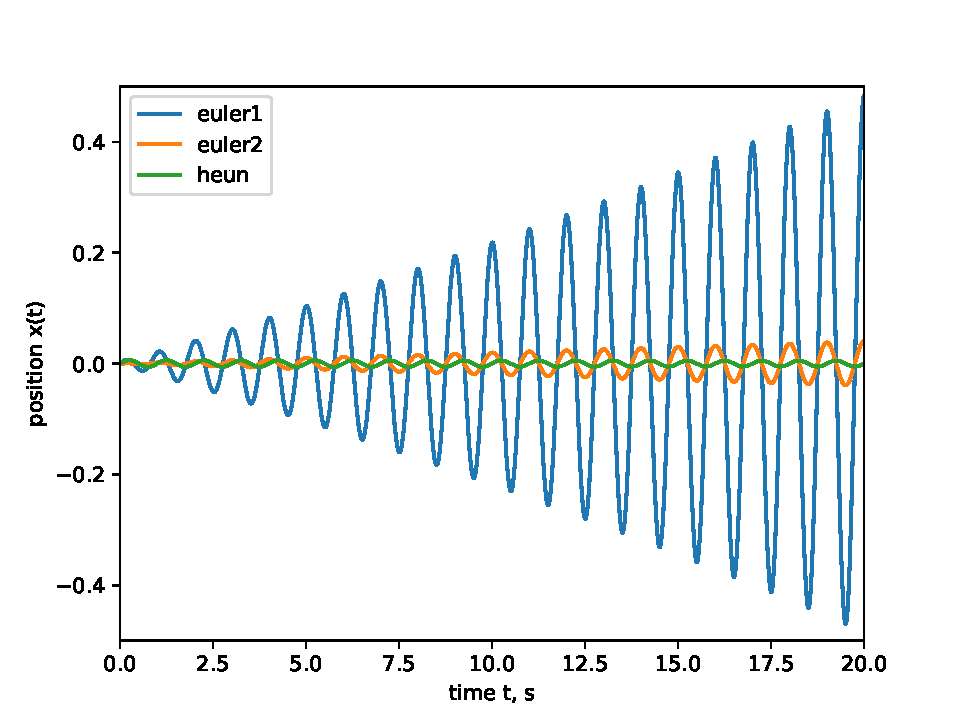
\includegraphics[width=\textwidth]{figures/eul12+heun-theory.pdf}
			\caption{Deviation from the theoretical solution.\label{subfig:sho-dev}}
		\end{subfigure}
		\hfill

		\hfill
		\begin{subfigure}[t]{0.48\textwidth}
			\centering
			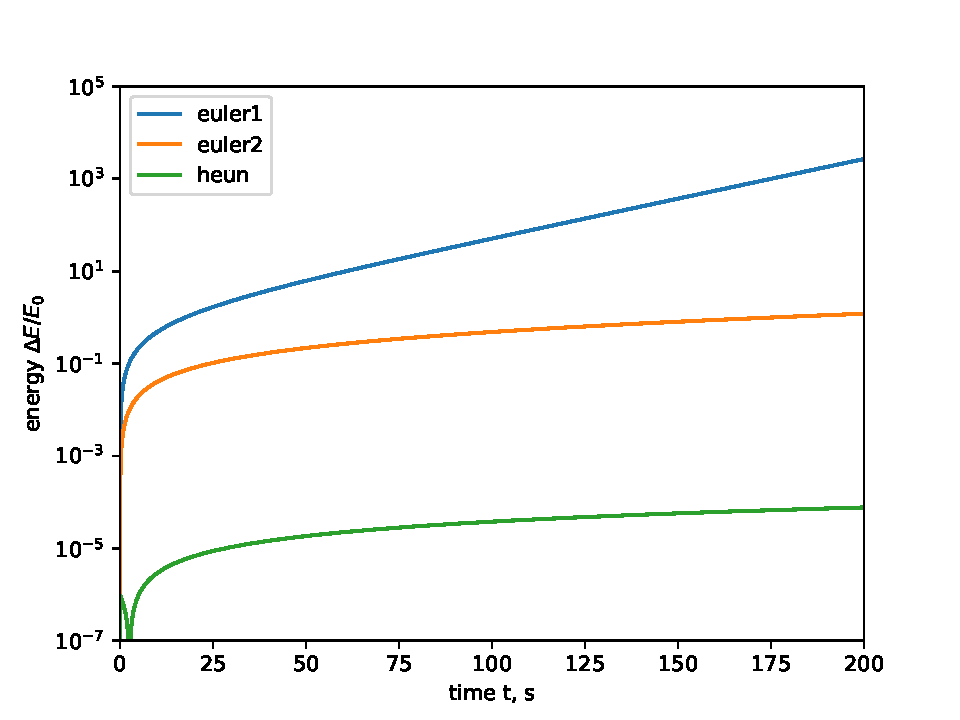
\includegraphics[width=\textwidth]{figures/eul12+heun+energy.pdf}
			\caption{Energy deviation $\Delta E/E_0$ for first three methods.\label{subfig:sho-energy1}}
		\end{subfigure}
		\hfill
		\begin{subfigure}[t]{0.48\textwidth}
			\centering
			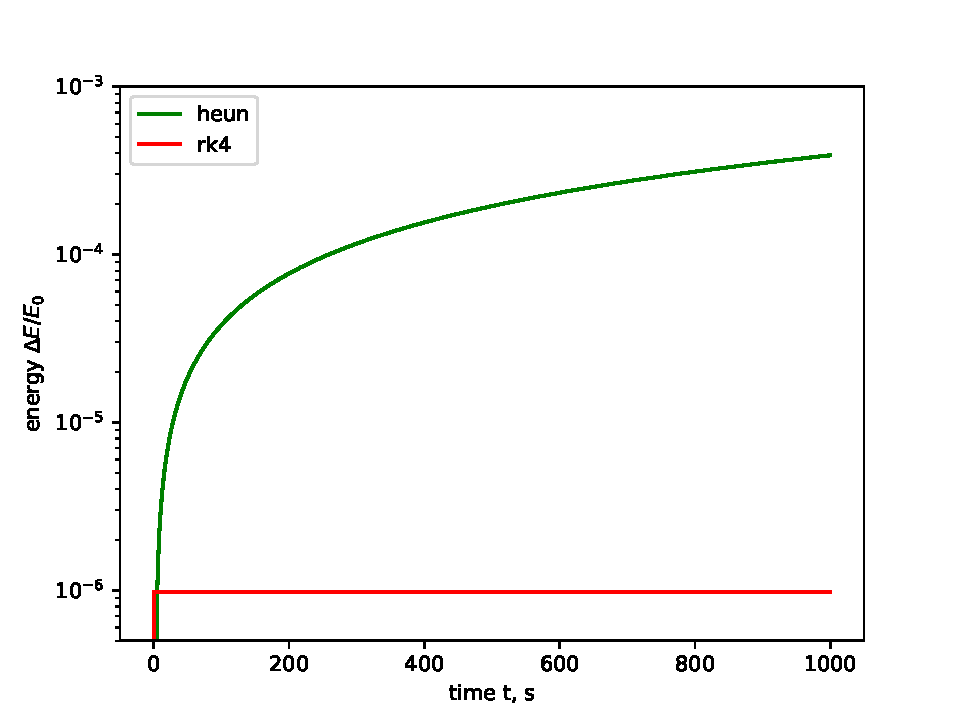
\includegraphics[width=\textwidth]{figures/heunRK4+energy.pdf}
			\caption{Energy deviation $\Delta E/E_0$ for heun and rk4.\label{subfig:sho-energy2}}
		\end{subfigure}
		\hfill
		\caption{Test runs of SHO integrated with different methods. Blue line is for Euler's method integrated with step \SI{1}{ms}, yellow line for Euler's method integrated with step \SI{0.1}{ms}, green line is for Heun's method with step \SI{1}{ms}, and red line is for RK4 method with step \SI{1}{ms}.\label{fig:sho-integration}}
	\end{figure}

	Results are presented in Figure \ref{fig:sho-integration}. In \ref{subfig:sho-pos} (first 20 periods of oscillation displayed), we see the calculated position by the three methods \eulerOne{}, \eulerTwo{}, and \heun{}. It is immediately clear that \eulerOne{} goes off in the solution pretty quickly. This is confirmed in \ref{subfig:sho-dev}, where we can have a better look at how the numerical solution deviates from the actual one - \eulerOne{} gains an additional half amplitude in 20 periods, while the other two methods oscillate about zero with \heun{} having the smaller error. To compare for the whole time of integration and compare these three runs with \rkFour{}, we plot the relative energy deviation compared to the theoretical value of $2E_0 = \omega^2 \times 1$ on a logarithmic scale. As it can be seen in \ref{subfig:sho-energy1} and \ref{subfig:sho-energy2}, the energy for the first three runs grows exponentially with time after some moment with different exponents, while the fourth run \rkFour{} keeps almost a constant value of energy --- the change in energy between $t_0=\SI{0}{s}$ and $t_1=\SI{100}{s}$ is:
	\begin{equation}
		\frac{\big| E(t_1) - E(t_0) \big|}{E(t_0)} \approx 9.755 \times 10^{-7}.
	\end{equation}

	With these results in mind, we make the clear choice for a method and continue forwards using the Runge-Kutta 4th order method in all of the following chapters.


\subsection{Dimensionless equation for the white dwarf}
	%		- Normalization - take into form that is implemented in the program
	To calculate values with the computer, we will go to dimensionless quantities in the differential equation. Introduce the following substitutions:
	\begin{equation}
		\rho = \rhoCentre \theta, \quad r = \ell \xi, \quad m = \rhoCentre (\SI{1}{m^3}) \mu \text{, therefore } \vec{y}(r) = \begin{pmatrix}\rho(r) \\ m(r)\end{pmatrix} \rightarrow \vec{\eta}(\xi) = \begin{pmatrix}\theta(\xi)\\\mu(\xi)\end{pmatrix}.
	\end{equation}
	We also specify the length $\ell$ by the equation $\frac{4}{3}\pi \ell^3 = \SI{1}{m^3}$, which gives a value of $\ell \approx 0.62 \sim \SI{1}{m}$. This will be useful to make some cancellations in the coefficients in the final form of the differential equation for $\vec{\eta}$. The initial conditions therefore become $\vec{\eta}(1) = \left( \theta(1), \mu(1)\right) = \left(1.0, 1.0 \right)$.

	For \eqref{eqn:mass-dEq}  the conversion is straightforward:
	\begin{equation}
		\frac{\rhoCentre \dd \mu}{\ell \dd \xi} = 4 \pi \ell^2 \xi^2 \rhoCentre \theta \quad \Rightarrow \quad \frac{\dd \mu}{\dd \xi} = 3 \xi^2 \theta.
	\end{equation}

	For the $\theta$ equation we have to take into consideration the regime we operate in --- whether we solve for a relativistic or non-relativistic equation of state. Firstly, write equations in \eqref{eqn:fermi-mtm} using the new coordinates we have introduced:
	\begin{equation}\label{eqn:fermi-mtm-new}
		\fermiMtm = \left( \frac{h^3 \rhoCentre}{16 \pi \massProton}\right)^{\sfrac{1}{3}} \theta^{\sfrac{1}{3}} , \quad \frac{\dd \fermiMtm}{\dd \rho} = \frac{1}{3} \left( \frac{h^3}{16 \pi \massProton \rhoCentre^2}\right)^{\sfrac{1}{3}} \theta^{-\sfrac{2}{3}}.
	\end{equation}
	Now substitute \eqref{eqn:pressure-both} in \eqref{eqn:hydrostat-equil-rhor} using \eqref{eqn:fermi-mtm-new}. After some algebra with the constants, the final result is the following:
	\begin{equation}
		\frac{\dd \theta}{\dd \xi} = K_1 \frac{\mu \theta^{\sfrac{1}{3}}}{\xi^2} \begin{cases}
			1 & \text{ in the non-relativistic case}\\
			\left(1 + K_2 \theta^{\sfrac{2}{3}}\right)^{\sfrac{1}{2}} & \text{ in the relativistic case}
		\end{cases},
	\end{equation}
	where the constants $K_1$ and $K_2$ are given by
	\begin{equation}
		K_1 = - 2^{\sfrac{13}{3}} \pi \gravconst \massElectron \massProton^{\sfrac{5}{3}} \rhoCentre^{\sfrac{1}{3}} h^{-2} , \quad \quad K_2 = \frac{1}{\massElectron^2 c^2} \left( \frac{3h^3 \rhoCentre}{16 \pi \massProton} \right)^{\sfrac{2}{3}}.
	\end{equation}
	We have completed the task of bringing the equation to normalized coordinates. This is the setup used in implementing the code for the white dwarf ODE wrapper presented in Appendix \ref{subapp:mainODE}.

\subsection{Convergence and number of intervals}\label{subsec:convergence}
	%		- Convergence => determine number of steps
	What is left is to choose the coarseness in the grid of $\xi$. We know that for some $\Delta \xi$ small enough, the answers will converge to $\approx$ a single value. To find the number of intervals (NoI) at which the result converges, we make experimental runs at three different $\rhoCentre$ --- $10^6$, $10^{10}$, and $10^{14}$ \si{kg.m^{-3}} (this spans the range for which we run the experiment later), and test for an NoI in the range $\left\{a \times 10^b \mid a \in \{1,2,4,8\}, b \in \{2,3,\ldots 8\}\right\}$. The maximal radius is set to $8.1 \times 10^7$ in units of $\xi$ since this turns out to be about the maximum physical radius a white dwarf can be for the range of $\rhoCentre$ we test. Both the non-relativistic and relativistic cases are considered.

	\begin{figure}[!htb]
		\centering
		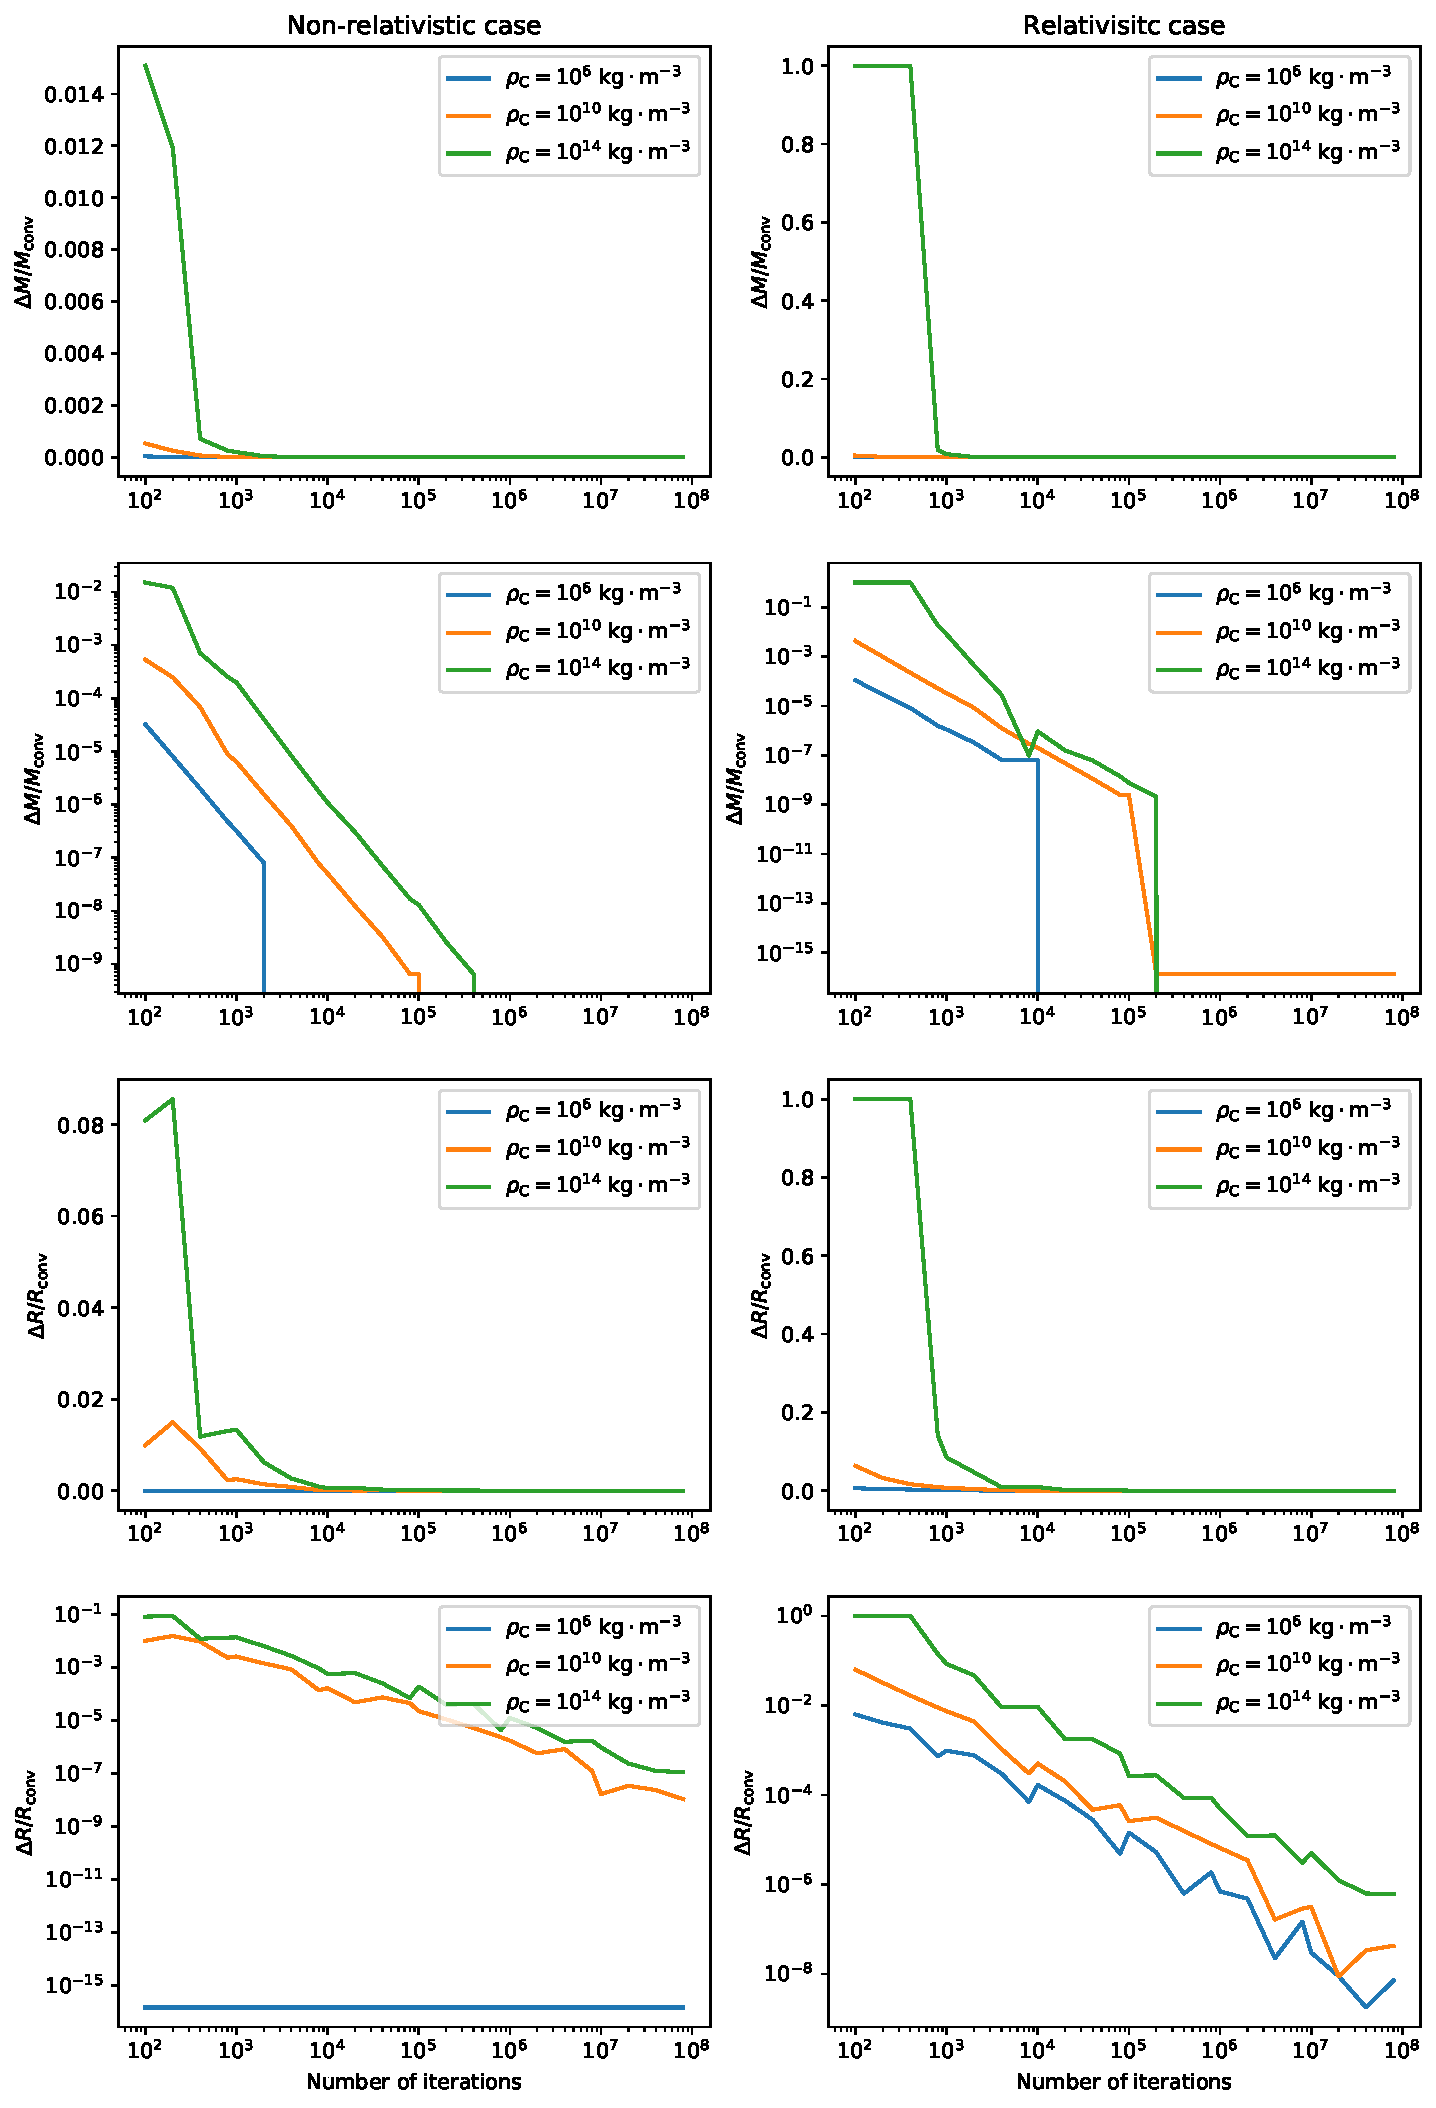
\includegraphics[height=0.87\textheight,keepaspectratio]{figures/convergencePlot.pdf}
		\caption{Plot of convergence for three central spanning the tested range of $\rhoCentre$ in both non-relativistic (left column) and relativistic (right column) cases. As can be seen, convergence is slower in the relativistic case; after $10^6$ intervals good accuracy is achieved in both cases for both mass and radius values. The values $M_\textrm{conv}, R_\textrm{conv}$ are computed as the average of the last three values; $\Delta M = \left| M - M_\mathrm{conv}\right|$ and $\Delta R = \left| R - R_\mathrm{conv}\right|$. Odd rows have a linear y-axis, even rows are the same plot with a logarithmic y-axis.\label{fig:convergence-results}}
	\end{figure}

	The results are presented in Figure \ref{fig:convergence-results}. We use the relative error in computed value with respect to the converged value. The latter is estimated as the average of the last three values in the calculation, i.e. for NoI $2 \times 10^8$, $4 \times 10^8$, and $8 \times 10^8$; the result is $M_\textrm{conv}, R_\textrm{conv}$. The relative error is given by:
	\begin{equation}
		\frac{\Delta M}{M_\mathrm{conv}} = \frac{\left| M - M_\mathrm{conv}\right|}{M_\mathrm{conv}}, \quad \frac{\Delta R}{R_\mathrm{conv}} = \frac{\left| R - R_\mathrm{conv}\right|}{R_\mathrm{conv}}.
	\end{equation}
	
	What we aim for in our choice for the number of intervals is: on the one side, a low enough number so the computation does not take too long, and on the other side, a high enough number so an acceptable accuracy is achieved. From the logarithmic plots for the mass and the radius determination, we see that the computed value does not really converge to a specific point; it does, however, reduce its error exponentially fast. Let us choose the desired accuracy of below $10^{-5} = 0.001 \%$, given that our model is not very accurate. From the logarithmic plots again we see that this is satisfied for $\text{NoI} \geq 2 \times 10^6$. Therefore, we can use this value as the NoI with a good compromise between speed and accuracy.

\section{Results and discussion}\label{sec:results-and-discussion}
	We begin by choosing the parameters of the simulation. As discussed in Section \ref{subsec:convergence}, we use the RK4 method of integration. The range of integration in $\xi$ will be $\left[ 1, \num{8.1e7}\right]$ with $2 \times 10^6$ intervals (we implement the white dwarf wrapper in this way to speed up the procedure, see Appendix \ref{subapp:mainODE}). This corresponds to physical dimensions of approximately $r \in \left[\SI{0.6}{m}, \SI{5e7}{m}\right]$ and a step size of $\Delta r = \SI{25}{m}$, which makes sure we do not reach the end of the range before the end of the star.

	For the central density $\rhoCentre$ we are tasked to study the range $10^6 < \rhoCentre < \SI{5e14}{kg.m^{-3}}$, so we set up to test using the following values: $\rhoCentre \in \left\{a \times 10^b \mid a = 1,2,\ldots,9 ; b = 6,7, \ldots, 14\right\}$. The results are presented in Figures \ref{fig:radius-rhoC}, \ref{fig:mass-rhoC}, and \ref{fig:radius-mass}. We have chosen logarithmic plots for the first two plots to better highlight the similar behaviour at low densities and the different behaviour at high densities.
	\begin{figure}[!htb]
		\centering
		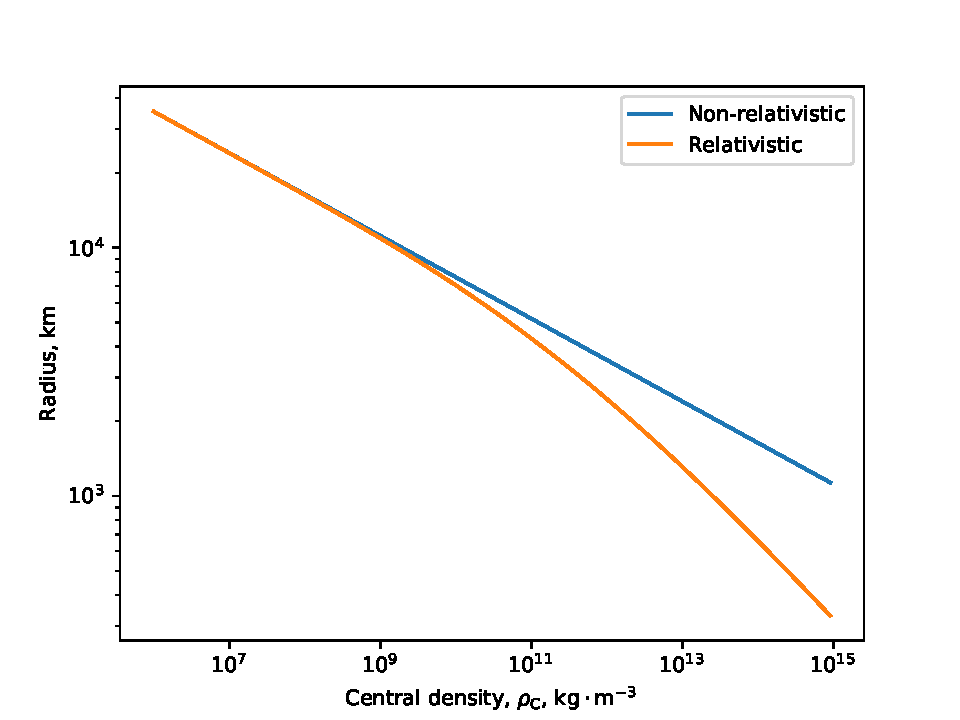
\includegraphics[height=0.3\textheight]{figures/radius-rhoC.pdf}
		\caption{Radius of a white dwarf $R$ in km as a function of central density $\rhoCentre$.\label{fig:radius-rhoC}}
	\end{figure}
	\begin{figure}[!htb]
		\centering
		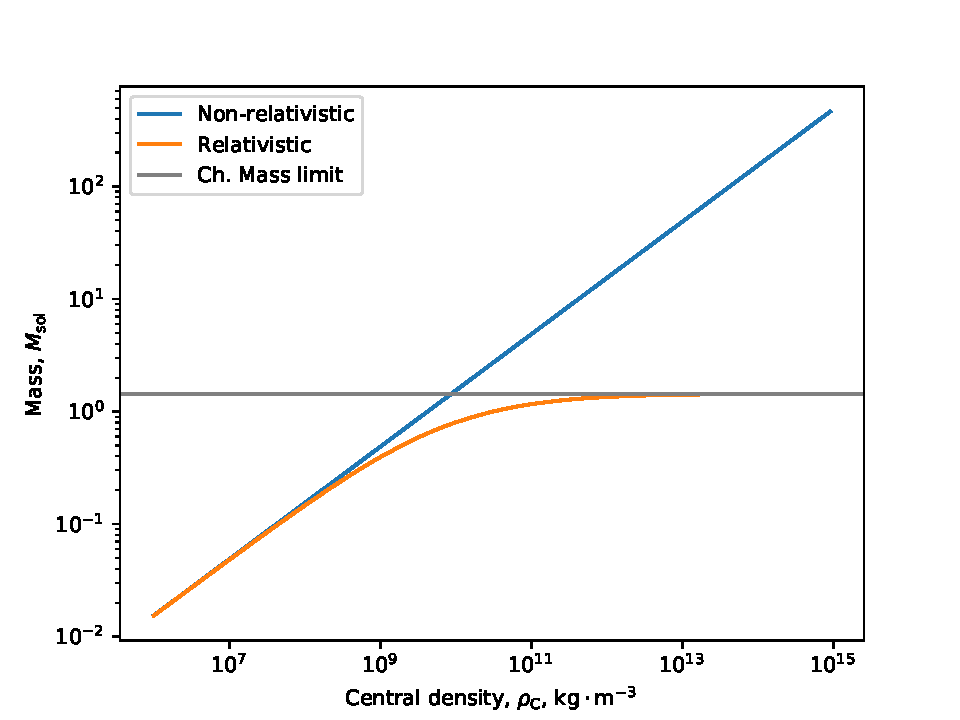
\includegraphics[height=0.3\textheight]{figures/mass-rhoC.pdf}
		\caption{Mass of a white dwarf star $M$ in solar masses as a function of central density$\rhoCentre$. Note the Chandrasekhar mass limit.\label{fig:mass-rhoC}}
	\end{figure}
	\begin{figure}[!htb]
		\centering
		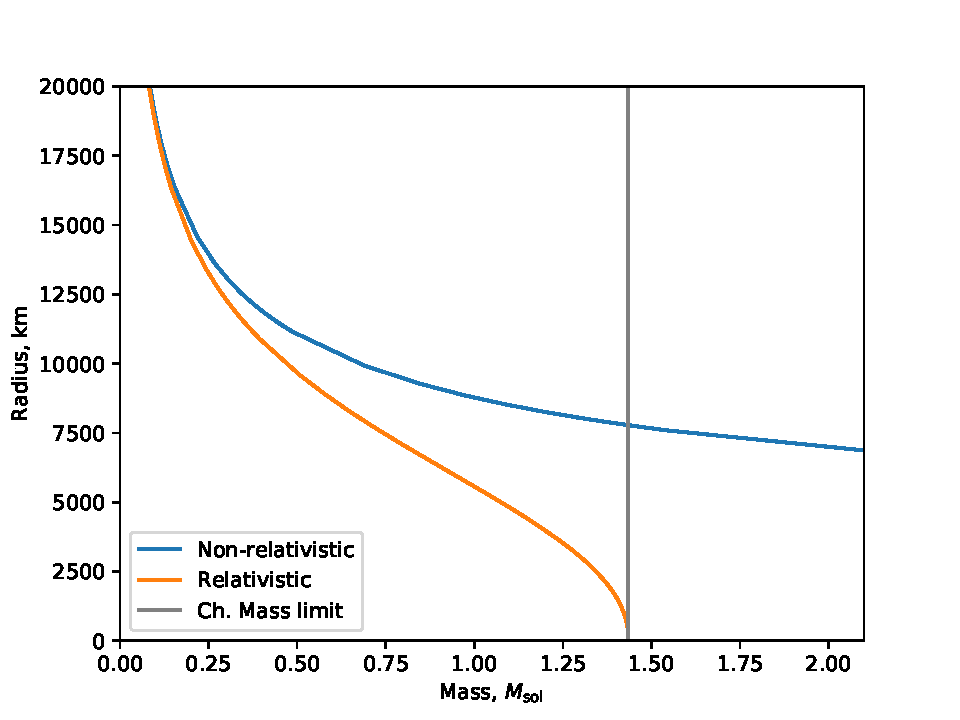
\includegraphics[height=0.3\textheight]{figures/radius-mass.pdf}
		\caption{Radius of a white dwarf $R$ in km as a function of the mass $M$ in solar masses. Note the Chandrasekhar mass limit.\label{fig:radius-mass}}
	\end{figure}
	 
	In Figure \ref{fig:radius-rhoC} and \ref{fig:mass-rhoC} we can see that at central densities $ \rhoCentre \approx 10^8$ the results for radius and mass start to deviate. The non-relativistic values follow an exponential relationship, as one might have predicted from \eqref{eqn:pressure-both} and \eqref{eqn:hydrostat-equil-rhor}. The relativistic case, on the other hand, exhibits more interesting behaviour. At higher densities, the mass tends to a single maximum value --- the \emph{Chandrasekhar mass}, which can be seen in Figures \ref{fig:mass-rhoC} and \ref{fig:radius-mass}. This implies that the theoretical model of a white dwarf cannot properly describe objects with higher mass.

	\subsection{Compact objects}
	White dwarfs are part of the more general framework of compact objects as end stages in stellar evolution, which also include neutron stars and black holes. These objects are the final result of stellar evolution. In which one a star settles is almost completely determined by its initial mass during the stable stage on the Main sequence. 
	
	Low to medium mass stars ($0.6 M_{\astrosun} \lesssim M \lesssim 8 M_{\astrosun}$) usually evolve by hydrogen burning joined by helium burning in the red giant stage. Since their carbon cores are not massive enough to ignite, the stars contract again and the strong stellar wind expels all surrounding gas to form a planetary nebula with a hot central star, which in turn cools down to a white dwarf. These white dwarfs are usually carbon and oxygen-rich.

	High mass stars ($M \gtrsim 8 M_{\astrosun}$) have massive enough cores to ignite further production of heavier elements via the alpha and triple alpha processes. After most of the fuel is burned through and a dense iron core has formed, they undergo a similar process of implosion in which the core rapidly compactifies (in some edge cases about $8 M_{\astrosun}$ only partial fusion of carbon occurs, they settle to a white dwarf state). In this case, however, the core mass has passed the (effective) Chandrasekhar limit and electron degeneracy pressure cannot support the equilibrium. Thus, the core collapses further to a neutron star or a black hole (the exact mass threshold for neutron stars is estimated to be between $2 M_{\astrosun}$ and $3 M_{\astrosun}$).

	It is the discovery of this limit in \cite{Chandrasekhar1931}, however, that started the whole further theoretical study of the topic of compact objects. In the following year, the neutron was discovered, and Landau published a paper that discussed a more precise calculation of the white dwarf mass limit and pondered the nature of heavier stars. This laid the groundwork for further discoveries in the 20th century.

	\subsection{Binary systems}
	Additionally, white dwarfs are often part of binary or multiple systems (about a third of all star systems are multiple systems). In the case the white dwarf is part of a very close binary, there is an accretion of mass to the surface of the white dwarf to a thin dense atmosphere layer atop the surface of the star. This atmosphere, usually comprised of hydrogen, is heated up by the star, which causes the ignition of runaway fusion. This is observed as a sudden flash of light - a \emph{nova}.

	If there is accretion from a more massive companion to a carbon-oxygen white dwarf (heavier elements support further collapse since more energy is needed for their ignition), this can cause its mass to increase beyond the Chandrasekhar limit and ignite carbon fusion in the centre of the white dwarf due to compressional heating. This results in the destruction of the star and is believed to be the physical model behind Type Ia \emph{supernovae}.
	
	These two phenomena further highlights the critical mass limit of existence for white dwarfs. Without it, the above would not be observed in nature.

\section{Summary}\label{sec:summary}
	In this practical, we study the structure of white dwarf stars by numerically solving the equations of equilibrium. For a white dwarf star, the equilibrium is supported by the electron degeneracy pressure. We derive these equations in Section \ref{sec:theroy-white-dwarfs}, differentiating between the cases of non-relativistic and relativistic electrons. Additionally, we consider the ultrarelativistic limit and anticipate the result of calculations --- a limit to white dwarf mass in the case of relativistic electrons.
	
	We choose to solve these equations as an initial value problem, where the starting point is a small region at the centre of the star. In Section \ref{sec:numerical-approach}, we compare the Euler, Heun, and Runge-Kutta 4th order (RK4) methods, which resulted in our choice to use the RK4 for solving the white dwarf equations. Then we introduce a transformation of variables to dimensionless quantities, after which we test the convergence of white dwarf mass and radius for a sample of central density values. We conclude that when the tested interval for radial distance in dimensionless units is $\xi \in \left[ 1, \num{8.1e7}\right]$ with $2 \times 10^6$ intervals we have a good compromise between accuracy and speed (this corresponds to physical dimensions of approximately $r \in \left[\SI{0.6}{m}, \SI{5e7}{m}\right]$ and a step size of $\Delta r = \SI{25}{m}$).

	We present the solution to the white dwarf equation in Section \ref{sec:results-and-discussion}. We note the difference of solutions between the non-relativistic and relativistic equation of state as the central density grows, seen in Figures \ref{fig:radius-rhoC} and \ref{fig:mass-rhoC}. There we also discuss the implications of the existence of the \emph{Chandrasekhar limit} and the place of white dwarfs in the evolutionary track of stars as an end stage of medium mass stars $M \lesssim 8 M_{\astrosun}$, compared to other compact objects (neutron stars and black holes). Finally, we note some other astrophysical phenomena which occur due to the special properties of white dwarfs --- novae and supernovae Type Ia.

	While this project takes steps towards a numerical solution of white dwarf equations, we have made some major assumptions along the way with regards to the physics. Among the effects to be taken into account in a further study are the following:
	\begin{itemize}
		\item The interaction of electrons with their surroundings: we can introduce magnetic fields and the electrostatic interaction in the force balance equations, which modifies the white dwarf equation.
		\item Chemical composition: since stars form an onion-like structure of elements in their cores, the mean molecular weight per electron $\mu_\mathrm{e}$ varies slightly, which changes the constant factors in the equation for the white dwarf.
		\item Effects of General Relativity should also be taken into account. White dwarfs are compact objects, so as the density grows larger, the effects are more and more significant.
		\item We assumed that the star is in a complete stationary equilibrium state. However, we also have to consider the cases where the star might be rotating (a compact object can have a significant rotation speed due to conservation of angular momentum) or pulsating, which can disturb the conditions in the centre.
	\end{itemize}
	An introductory account of some of these effects can be found in e.g. \cite{Sagert2005}, while a more standard and in-depth textbook exposition to the topic can be found in \cite{Shapiro1991}.

	Additionally, there is room for improvement in the computational methods employed as well. The fairly simple RK4 method can be modified to have a varying step size that self-corrects depending on the derivative at a given point. That way the calculations can skip over a region with small a small gradient by increasing the step size, and decrease the step size to get a more accurate value for the change in a region with a big gradient. Another direction of improvement would be to change from RK4 to another, a more sophisticated method that has better accuracy and faster computational time like the Bulirsch-Stoer method. This would be especially helpful if the system of differential equations to be solved was much more complex in its behaviour. A good introductory text on the subject is \cite{Press2007},~Chapter~17.

\bibliographystyle{agsm}
\renewcommand{\bibname}{References}
\bibliography{test}

\newpage
\appendix
\section{Source code}\label{app:source-code}

The structure of the code has been guided by the guidance set in \cite{OxfPhys2020}. Additionally, \cite{Press2007} has had some influence on general code structure. The documentation for the main ODE solver is in the Python code. A copy in an online repository can be found \href{https://github.com/lyubomirShoylev/co31-white-dwarf}{here}.

\subsection{Main ODE facilities}\label{subapp:mainODE}
\inputminted[frame=single, linenos, python3]{python}{../modules/ode.py}
\inputminted[frame=single, linenos, python3]{python}{../modules/whiteDwarf.py}
\inputminted[frame=single, linenos, python3]{python}{../modules/integrators.py}
\inputminted[frame=single, linenos, python3]{python}{../modules/derivatives.py}

\subsection{Code to run the experiment and testing procedures}
\inputminted[frame=single, linenos, python3]{python}{../main.py}
\inputminted[frame=single, linenos, python3]{python}{../convergence.py}
\inputminted[frame=single, linenos, python3]{python}{../methodEval.py}
\inputminted[frame=single, linenos, python3]{python}{../mainPlots.py}
\end{document}